\ifdefined\iscombined
	\lecturetitle{Gears and Impedance Reflection}
\else
\documentclass{article}
\usepackage{xparse}
\usepackage{changepage}
\usepackage{listings}
\usepackage{amsthm}
\usepackage{comment}
\usepackage{amsmath}
\usepackage{braket}
\usepackage{amsfonts}
\usepackage{sectsty}
\usepackage{hyperref}
\usepackage{fancyhdr}
\usepackage[top=1in,bottom=1in,left=1in,right=1in]{geometry}
\usepackage{float}
\usepackage{graphicx}
\usepackage{mathtools}
\usepackage{tikz}
\usetikzlibrary{arrows,calc,patterns,decorations.pathmorphing,decorations.markings,shapes.geometric}
\usepackage{circuitikz}

\date{
	\vspace{-.75em}
	{\large \today}
}

\title{
	\vspace*{-1.5em}
	{\Huge Lecture 12} \\
	\vspace{-1em}
	\rule{\textwidth/4}{.01em} \\
	\vspace{-.25em}
	{\Large Gears and Impedance Reflection}
	\vspace{-.75em}
}

\author{
	{\large Matthew Farah}
}

\hypersetup{
	colorlinks=true,
	linkcolor=blue,
	filecolor=magenta,
	urlcolor=blue,
	citecolor=blue,
	anchorcolor=blue
}

\fancyhead{}
\fancyhead[L]{\today}
\fancyhead[R]{Lecture 12 - Gears and Impedance Reflection}

\setlength{\parindent}{0cm}

\newcounter{example}
\renewcommand{\theexample}{\arabic{example}}

\newenvironment{example}[1][]{
	\refstepcounter{example}
	\begin{adjustwidth}{1.5em}{}
	\vspace{1em}
	\noindent\textbf{\ifx&#1&Example \theexample:\else Example \theexample \ (#1):\fi}
	\ignorespaces
}{
	\vspace{.5em}
	\end{adjustwidth}
}

\newenvironment{solution}{
	\vspace{.5em}
	\par
	\begin{adjustwidth}{1.5em}{}
	\textbf{{Solution:}}
	\par
	\vspace{.5em}
}{
	\vspace{1em}
	\end{adjustwidth}
}

\newcounter{subexample}
\renewcommand{\thesubexample}{\alph{subexample}}

\newenvironment{subexample}{
	\setcounter{step}{0}
	\refstepcounter{subexample}
	\vspace{1em}\par\noindent
	\begin{adjustwidth}{1.5em}{}
	\noindent\textbf{(\thesubexample)}
	\ignorespaces
}{
	\par
	\vspace{1em}
	\end{adjustwidth}
}

\renewenvironment{proof}{
	\vspace{.5em}\par\noindent
	\begin{adjustwidth}{1.5em}{}
	\emph{Proof:}\par\vspace{1em}
	\setlength{\parindent}{0cm}
}{
	\end{adjustwidth}
}

\newtheorem{theorem}{Theorem}

\renewenvironment{theorem}[1][]{
	\refstepcounter{theorem}
	\vspace{1em}\par\noindent
	\begin{adjustwidth}{1.5em}{}
	\noindent\textbf{\ifx&#1&Theorem \thetheorem:\else Theorem \thetheorem \ (#1):\fi}
	\ignorespaces
}{
	\vspace{.5em}
	\end{adjustwidth}
}

\newtheorem{lemma}{Lemma}

\renewenvironment{lemma}[1][]{
	\refstepcounter{lemma}
	\vspace{1em}\par\noindent
	\begin{adjustwidth}{1.5em}{}
	\noindent\textbf{\ifx&#1&Lemma \thelemma:\else Lemma \thelemma \ (#1):\fi}
	\ignorespaces
}{
	\vspace{.5em}
	\end{adjustwidth}
}

\makeatother
\makeatletter

\newcounter{step}
\renewcommand{\thestep}{\Roman{step}}

\newenvironment{step}{
	\refstepcounter{step}
	\vspace{1em}\par\noindent
	\ignorespaces\noindent\textbf{(\thestep)}
	\ignorespaces
}{
	\par
	\vspace{1em}
}

\sectionfont{\fontsize{12}{12}\bfseries}
\subsectionfont{\fontsize{10}{12}\normalfont}
\subsubsectionfont{\fontsize{10}{12}\normalfont}

\begin{document}

\maketitle
\pagestyle{fancy}

\fi

\begin{itemize}
	\item Gears are used frequently in rotational systems. A sequence of interconnected gears is called a gear train.
	\item The number of teeth a gear has is always assumed to be an integer, and is denoted $N$.
	\item The number of teeth a gear has is proportional to its radius: $N \propto r$.
	\item When gears in contact rotate, that rotation covers the same distance on each gear's circumference, irrespective of the number of gears.
\end{itemize}

\begin{example}
	What is the relationship between the applied torque $T(t)$ and the induced torque $T_2(t)$ in the following system?

	\vspace{1em}

	\begin{figure}[H]
		\centering
		\begin{tikzpicture}[>=stealth]
			\newcommand{\AxisRotator}[1][rotate=0]{
				\tikz [x=0.25cm,y=0.60cm,line width=.2ex,-stealth,#1] \draw (0,0) arc (-150:150:1 and 1);
			}

			\draw [thick] (0,0.8) -- (3,0.8);
			\draw [thick] (3,1.2) -- (3,0.4);
			\node [anchor=south west] at (3.1,1.0) {$N_1$};

			\draw [thick] (3,-1.8) -- (3,-1);
			\node [anchor=north east] at (2.9,-.8) {$N_2$};
			\draw [thick] (3,-1.4) -- (6,-1.4);

			\draw ($(1.5, 0.8)$) node[label={[label distance = -3pt, font=\scriptsize]above:{$T(t)$}}] {\AxisRotator[rotate = 180, scale=.5]};
			\draw ($(4.5, -1.4)$) node[label={[label distance = -3pt, font=\scriptsize]above:{$T_2(t)$}}] {\AxisRotator[rotate = 0, scale=.5]};
		\end{tikzpicture}
	\end{figure}
\end{example}

\begin{solution}
	We know that the applied torque will cause the top gear (pun intended) to rotate some angle $\theta_1(t)$. The top gear is in contact with the second gear, so rotating it by $\theta_1(t)$ will induce the other gear to rotate in the opposite direction by some angle $\theta_2(t)$. \\

	As stated earlier, we have that the distance covered by the top gear turning to an angle $\theta_1(t)$ equals the distance along the circumference covered by the bottom gear rotating to $\theta_2(t)$. Using the fact that the distance covered by one gear equals $r_i \theta_i(t)$, and noting that $r_1 \propto N_1$ and $r_2 \propto N_2$, we have that:

	\begin{equation*}
		\begin{array}{lrl}
			& r_1 \theta_1(t) =& r_2 \theta_2(t) \\\\
			\implies & \dfrac{r_1}{r_2} =& \dfrac{\theta_2(t)}{\theta_1(t)} \\\\
			\implies & \dfrac{N_2}{N_1} =& \dfrac{\theta_1(t)}{\theta_2(t)} \quad \ldots (1)
		\end{array}
	\end{equation*} \\

	We also know, by Newton's second law of motion, that $T_1(t) \theta_1(t) = T_2(t) \theta_2(t)$, and because:

	\begin{align*}
		\dfrac{T(t)}{T_2(t)} &= \dfrac{\theta_2(t)}{\theta_1(t)} \\
	\end{align*}

	We therefore have that:

	\begin{align*}
		\dfrac{T(t)}{T_2(t)} &= \dfrac{\theta_2(t)}{\theta_1(t)} = \dfrac{N_1}{N_2}
	\end{align*}
\end{solution}

\begin{itemize}
	\item The result above, that $\dfrac{T(t)}{T_2(t)} = \dfrac{N_1}{N_2}$, is very useful for all gear questions, and generalizes for any two gears (i.e. $\dfrac{T_i(s)}{T_j(s)} = \dfrac{N_i(s)}{N_j(s)}$).
	\begin{itemize}
		\item The above result also means we can move an impedence from great $j$ to gear $i$ by multiplying by $\left(\dfrac{N_i}{N_j}\right)^2$. \item This is known as impedance reflection.
	\end{itemize}
\end{itemize}

\begin{example}
	For the following system:

	\vspace{1em}

	\begin{figure}[H]
		\centering
		\begin{tikzpicture}[>=stealth]
			\newcommand{\AxisRotator}[1][rotate=0]{
				\tikz [x=0.25cm,y=0.60cm,line width=.2ex,-stealth,#1] \draw (0,0) arc (-150:150:1 and 1);
			}

			\draw [thick] (0,2.2) -- (3,2.2);
			\draw [thick] (3,1.8) -- (3,2.6);
			\node [anchor=south west] at (3.1,2.4) {$N_1$};
			\node [anchor=north west] at (3.1,2.0) {$J_1, D_1$};

			\draw [thick] (3,-0.4) -- (3,0.4);
			\node [anchor=north east] at (2.9,0.6) {$N_2$};
			\node [anchor=south east] at (2.9,-0.6) {$J_2, D_2$};
			\draw [thick] (3,0) -- (6,0);

			\draw [thick] (6,-0.4) -- (6,0.4);
			\node [anchor=south west] at (6.1,0.2) {$N_2$};
			\node [anchor=north west] at (6.1,-0.2) {$J_3$};

			\draw [thick] (6,-2.6) -- (6,-1.8);
			\node [anchor=north east] at (5.9,-1.6) {$N_3$};
			\node [anchor=south east] at (5.9,-2.8) {$J_4$};
			\draw [thick] (6,-2.2) -- (8,-2.2);

			\node (J5) [thick, cylinder, draw, fill=white, minimum width=0.9cm, minimum height=1.4cm] at (8,-2.2) {$J_5$};

			\draw ($(0.5, 2.2)$) node[label={[label distance = -3pt, font=\scriptsize]above:{$T(s)$}}] {\AxisRotator[rotate = 180, scale=.5]};
			\draw ($(1.6, 2.2)$) node[label={[label distance = -3pt, font=\scriptsize]above:{$\theta_1(s)$}}] {\AxisRotator[rotate = 180, dashed, scale=.5]};
			\draw ($(4.5, 0)$) node[label={[label distance = -3pt, font=\scriptsize]above:{$\theta_2(s)$}}] {\AxisRotator[rotate = 0, dashed, scale=.5]};
			\draw ($(7, -2.2)$) node[label={[label distance = -3pt, font=\scriptsize]above:{$\theta_3(s)$}}] {\AxisRotator[rotate = 180, dashed, scale=.5]};
		\end{tikzpicture}
	\end{figure}
\end{example}

\begin{subexample}
	Find the transfer function $G_1(s) = \dfrac{\Theta_1(s)}{T(s)}$.
\end{subexample}

\begin{solution}
	To find the transfer function, we must simplify our system down using impedance reflection to a single rotational system and then solve as normal. \\

	From our knowledge of rotational systems, we know that the impedance experienced by the first, second, and third pairs of gears respectively is given by:

	\begin{align*}
		J_1 s^2 + D_1 s, \quad (J_2 + J_3) s^2 + D_2 s, \quad (J_4 + J_5) s^2 \\
	\end{align*}

	So by reflecting the second and third impedances onto the first gear, we have that the impedance experienced by gear one is given by:

	\begin{align*}
		\left(J_1 + \left(\dfrac{N_1}{N_2}\right)^2 (J_2 + J_3) + \left(\dfrac{N_1}{N_3}\right)^2 (J_4 + J_5)\right) s^2 + \left(D_1 + \left(\dfrac{N_1}{N_2}\right)^2 D_2\right) s \\
	\end{align*}

	And by Newton's third law of motion:

	\begin{align*}
		\left(\left(J_1 + \left(\dfrac{N_1}{N_2}\right)^2 (J_2 + J_3) + \left(\dfrac{N_1}{N_3}\right)^2 (J_4 + J_5)\right) s^2 + \left(D_1 + \left(\dfrac{N_1}{N_2}\right)^2 D_2\right) s\right) \Theta_1(s) &= T(s) \\
	\end{align*}

	Therefore:

	\begin{align*}
		G_1(s) &= \dfrac{\Theta_1(s)}{T(s)} \\\\
		&= \dfrac{1}{\left(J_1 + \left(\dfrac{N_1}{N_2}\right)^2 (J_2 + J_3) + \left(\dfrac{N_1}{N_3}\right)^2 (J_4 + J_5)\right) s^2 + \left(D_1 + \left(\dfrac{N_1}{N_2}\right)^2 D_2\right) s}
	\end{align*}
\end{solution}

\begin{subexample}
	Find the transfer function $G_2(s) = \dfrac{\Theta_2(s)}{T(s)}$.
\end{subexample}

\begin{solution}
	As opposed to redoing all of our calculations from scratch, we simply need to realize that:

	\begin{align*}
		\dfrac{\Theta_2(s)}{T(s)} &= \dfrac{N_1}{N_2} \dfrac{\Theta_1(s)}{T(s)} = \dfrac{G_1(s)}{N_2 / N_1} \\
	\end{align*}

	Hence:

	\begin{align*}
		G_2(s) &= \dfrac{\Theta_2(s)}{T(s)} \\
			&= \dfrac{G_1(s)}{N_2 / N_1} \\
			&= \dfrac{1}{\left(\dfrac{N_2}{N_1} J_1 + \dfrac{N_1}{N_2} (J_2 + J_3) + \dfrac{N_1 N_2}{N_3^2} (J_4 + J_5)\right) s^2 + \left(\dfrac{N_2}{N_1} D_1 + \dfrac{N_1}{N_2} D_2\right) s}
	\end{align*}
\end{solution}

\begin{example}
	How many degrees of freedom does the following system have?

	\vspace{1em}

	\begin{figure}[H]
		\centering
		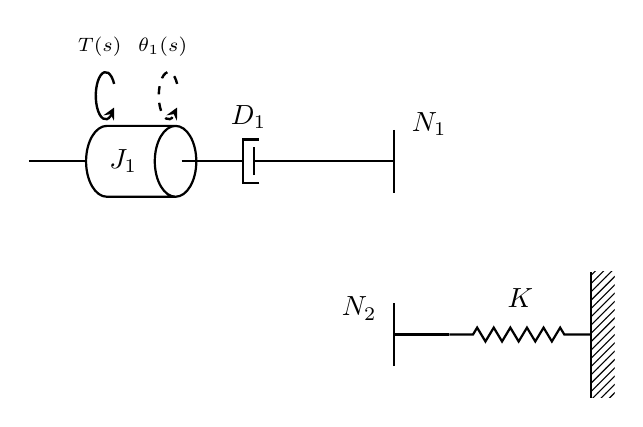
\begin{tikzpicture}[>=stealth]
			\tikzstyle{spring}=[thick,decorate,decoration={zigzag,pre length=0.3cm,post length=0.3cm,segment length=6}]
			\tikzstyle{damper}=[thick,decoration={markings,
				mark connection node=dmp,
				mark=at position 0.5 with
				{
					\node (dmp) [thick,inner sep=0pt,transform shape,rotate=-90,minimum width=15pt,minimum height=3pt,draw=none] {};
					\draw [thick] ($(dmp.north east)+(2pt,0)$) -- (dmp.south east) -- (dmp.south west) -- ($(dmp.north west)+(2pt,0)$);
					\draw [thick] ($(dmp.north)+(0,-5pt)$) -- ($(dmp.north)+(0,5pt)$);
				}
			}, decorate]

			\newcommand{\AxisRotator}[1][rotate=0]{
				\tikz [x=0.25cm,y=0.60cm,line width=.2ex,-stealth,#1] \draw (0,0) arc (-150:150:1 and 1);
			}

			\node (J1) [thick, cylinder, draw, minimum width=0.9cm, minimum height=1.4cm] at (1.2,0) {$J_1$};

			\draw [thick] (0,0) -- (J1.west);

			\draw [damper] ($(J1.east) + (-0.2, 0)$) -- ($(J1.east) + (1.5, 0)$) node[midway, above=8pt, fill=white] {$D_1$};

			\draw [thick] ($(J1.east) + (1.5, 0)$) -- ($(J1.east) + (2.5, 0)$);

			\draw [thick] ($(J1.east) + (2.5, 0.4)$) -- ($(J1.east) + (2.5, -0.4)$);
			\node [anchor=south west] at ($(J1.east) + (2.6, 0.2)$) {$N_1$};

			\draw [thick] ($(J1.east) + (2.5, -2.6)$) -- ($(J1.east) + (2.5, -1.8)$);
			\node [anchor=north east] at ($(J1.east) + (2.4, -1.6)$) {$N_2$};

			\draw [thick] ($(J1.east) + (2.5, -2.2)$) -- ($(J1.east) + (3.2, -2.2)$);

			\draw [spring] ($(J1.east) + (3.2, -2.2)$) -- ($(J1.east) + (5.0, -2.2)$) node[midway, above=6pt, fill=white] {$K$};

			\draw [thick] ($(J1.east) + (5.0, -3.0)$) -- ($(J1.east) + (5.0, -1.4)$);
			\fill [pattern=north east lines] ($(J1.east) + (5.0, -3.0)$) rectangle ($(J1.east) + (5.3, -1.4)$);

			\draw ($(J1.center) + (-0.3, 0)$) node[above=10pt, label={[label distance = -3pt, font=\scriptsize]above:{$T(s)$}}] {\AxisRotator[rotate = 180, scale=.5]};
			\draw ($(J1.center) + (0.5, 0)$) node[above=10pt, label={[label distance = -3pt, font=\scriptsize]above:{$\theta_1(s)$}}] {\AxisRotator[rotate = 180, dashed, scale=.5]};
		\end{tikzpicture}
	\end{figure}
\end{example}

\begin{solution}
	Very counter-intuitively, this system actually has three degrees of freedom due to the viscous damper between $J_1$ and the first gear. \\

	\emph{Note to self: Should elaborate}
\end{solution}

\ifdefined\iscombined
	\newpage
\else
	\end{document}
\fi
